\documentclass[
	% -- opções da classe memoir --
	12pt,				% tamanho da fonte
	openright,			% capítulos começam em pág ímpar (insere página vazia caso preciso)
	oneside,			% para impressão em recto e verso. Oposto a oneside
	a4paper,			% tamanho do papel. 
	% -- opções da classe abntex2 --
	chapter=TITLE,		% títulos de capítulos convertidos em letras maiúsculas
	section=TITLE,		% títulos de seções convertidos em letras maiúsculas
	subsection=TITLE,	% títulos de subseções convertidos em letras maiúsculas
	subsubsection=TITLE,% títulos de subsubseções convertidos em letras maiúsculas
    subsubsubsection=TITLE,% títulos de subsubsubseções convertidos em letras maiúsculas
	% -- opções do pacote babel --
	english,			% idioma adicional para hifenização
    french,
    spanish,
	brazil				% o último idioma é o principal do documento
	]{utfprtex2}



% ---
% Pacotes básicos 
% ---

\usepackage[utf8]{inputenc}		% Codificacao do documento (conversão automática dos acentos)
\usepackage{svg}
\usepackage[bf]{caption}       %NEGRITO LEGENDA
\usepackage{booktabs}
\usepackage{nimbussans}
\renewcommand*\familydefault{\sfdefault} %% Only if the base font of the document is to be sans serif
\usepackage[T1]{fontenc}
\usepackage{subfigure}           % Habilita o uso de Sub_Figuras

\usepackage{blindtext}
\usepackage{lastpage}			% Usado pela Ficha catalográfica
\usepackage{indentfirst}		% Indenta o primeiro parágrafo de cada seção.
\usepackage{color}				% Controle das cores
\usepackage{graphicx}			% Inclusão de gráficos
\usepackage{microtype} 			% para melhorias de justificação

\usepackage{enumerate}          %listas numeradas i,ii,iii, etc
\usepackage{enumitem}
	
% ---
		
% ---
% Pacotes adicionais, usados apenas no âmbito do Modelo Canônico do abnteX2
% ---
%\usepackage{lipsum}				% para geração de dummy text
% o pacote utfprtex2capatcc formata a capa para tcc. Se não for tcc não precisa usar

\usepackage{utfprtex2capatcc}
% ---

% ---
% Pacotes de citações
% ---
\usepackage[alf]{abntex2cite}	% Citações padrão ABNT
% ---

% ---
% Pacotes que não estavam no modelo
% ---
\usepackage{float} %para o posicionamento das figuras e tabelas
%\usepackage{soul}
 \usepackage{navigator}

\usepackage{amsmath}
\newcounter{matriz}
\newenvironment{matriz}{\refstepcounter{matriz}\equation} % usado para mudar numeração das equacoes
{\tag{\thematriz}\endequation}





% ---
% Informações de dados para CAPA e FOLHA DE ROSTO
% ---
\titulo{EXEMPLO DE UTILIZAÇÃO DO OVERLEAF: UM ESTUDO DE CASO NO TCC DA UTFPR PATO BRANCO}
\autor{Fulano de Tal}
\local{Pato Branco}
\data{ \the\year }
\orientador{Prof. Dr. Beltrano }
\coorientador{Prof. Dr. Sicrano }
\tipotrabalho{Trabalho de Conclusão de Curso}
% O preambulo deve conter o tipo do trabalho, o objetivo, 
% o nome da instituição e a área de concentração 
\preambulo{Trabalho de Conclusão do Curso de Engenharia Elétrica da Universidade Tecnológica Federal do Paraná - UTFPR, câmpus Pato Branco, apresentado como requisito parcial para obtenção do título de Engenheiro Eletricista.}
% ---


% ---
% Configurações de aparência do PDF final
\widowpenalty=10000
\clubpenalty=10000

% alterando o aspecto da cor azul
\definecolor{blue}{RGB}{41,5,195}

% informações do PDF
\makeatletter
\hypersetup{
     	%pagebackref=true,
		pdftitle={\@title}, 
		pdfauthor={\@author},
    	pdfsubject={\imprimirpreambulo},
	    pdfcreator={LaTeX with abnTeX2},
		pdfkeywords={abnt}{latex}{abntex}{abntex2}{trabalho acadêmico}, 
        %colorlinks=false,       		% false: boxed links; true: colored link
		colorlinks=true,       		
    	linkcolor=black,          	% color of internal links
    	citecolor=black,        		% color of links to bibliography
    	filecolor=black,      	% color of file links
		urlcolor=black,
		bookmarksdepth=4
}
\makeatother
% --- 

%Numerar equações em ordem numérica
\usepackage{chngcntr}

\counterwithout{equation}{chapter}

% --- 
% Espaçamentos entre linhas e parágrafos 
% --- 

% O tamanho do parágrafo é dado por:
\setlength{\parindent}{1.3cm}

% Controle do espaçamento entre um parágrafo e outro:
\setlength{\parskip}{0.2cm}  % tente também \onelineskip

% ---
% compila o indice
% ---
\makeindex
% ---

% ----
% Início do documento
% ----
\begin{document}
% Seleciona o idioma do documento (conforme pacotes do babel)
%\selectlanguage{english}
\selectlanguage{brazil}

% Retira espaço extra obsoleto entre as frases.
\frenchspacing 






% ----------------------------------------------------------
% ELEMENTOS PRÉ-TEXTUAIS
% ----------------------------------------------------------
% \pretextual

% ---
% Capa
% ---
\imprimircapa
% ---

% ---
% Folha de rosto
% (o * indica que haverá a ficha bibliográfica)
% ---
\imprimirfolhaderosto
% ---

% ---
% Inserir a ficha bibliografica
% ---

% Isto é um exemplo de Ficha Catalográfica, ou ``Dados internacionais de
% catalogação-na-publicação''. Você pode utilizar este modelo como referência. 
% Porém, provavelmente a biblioteca da sua universidade lhe fornecerá um PDF
% com a ficha catalográfica definitiva após a defesa do trabalho. Quando estiver
% com o documento, salve-o como PDF no diretório do seu projeto e substitua todo
% o conteúdo de implementação deste arquivo pelo comando abaixo:
%
% \begin{fichacatalografica}
%     \includepdf{fig_ficha_catalografica.pdf}
% \end{fichacatalografica}

% \begin{fichacatalografica}
% 	\sffamily
% 	\vspace*{\fill}					% Posição vertical
% 	\begin{center}					% Minipage Centralizado
% 	\fbox{\begin{minipage}[c][8cm]{13.5cm}		% Largura
% 	\small
% 	\imprimirautor
% 	%Sobrenome, Nome do autor
	
% 	\hspace{0.5cm} \imprimirtitulo  / \imprimirautor. --
% 	\imprimirlocal, \imprimirdata-
	
% 	\hspace{0.5cm} \pageref{LastPage} p. : il. (algumas color.) ; 30 cm.\\
	
% 	\hspace{0.5cm} \imprimirorientadorRotulo~\imprimirorientador\\
	
% 	\hspace{0.5cm}
% 	\parbox[t]{\textwidth}{\imprimirtipotrabalho~--~\imprimirinstituicao,
% 	\imprimirdata.}\\
	
% 	\hspace{0.5cm}
% 		1. Palavra-chave1.
% 		2. Palavra-chave2.
% 		2. Palavra-chave3.
% 		I. Orientador.
% 		II. Universidade xxx.
% 		III. Faculdade de xxx.
% 		IV. Título 			
% 	\end{minipage}}
% 	\end{center}
% \end{fichacatalografica}
% ---

% ---
% Inserir errata
% ---
% \begin{errata}
% Elemento opcional da \citeonline[4.2.1.2]{NBR14724:2011}. Exemplo:

% \vspace{\onelineskip}

% FERRIGNO, C. R. A. \textbf{Tratamento de neoplasias ósseas apendiculares com
% reimplantação de enxerto ósseo autólogo autoclavado associado ao plasma
% rico em plaquetas}: estudo crítico na cirurgia de preservação de membro em
% cães. 2011. 128 f. Tese (Livre-Docência) - Faculdade de Medicina Veterinária e
% Zootecnia, Universidade de São Paulo, São Paulo, 2011.

% \begin{table}[htb]
% \center
% \footnotesize
% \begin{tabular}{|p{1.4cm}|p{1cm}|p{3cm}|p{3cm}|}
%   \hline
%    \textbf{Folha} & \textbf{Linha}  & \textbf{Onde se lê}  & \textbf{Leia-se}  \\
%     \hline
%     1 & 10 & auto-conclavo & autoconclavo\\
%    \hline
% \end{tabular}
% \end{table}

% \end{errata}
% ---





% ---
% Inserir folha de aprovação
% ---

% Isto é um exemplo de Folha de aprovação, elemento obrigatório da NBR
% 14724/2011 (seção 4.2.1.3). Você pode utilizar este modelo até a aprovação do trabalho. Após isso, substitua todo o conteúdo deste arquivo por uma
% imagem da página assinada pela banca com o comando abaixo:

% \includepdf{folhadeaprovacao_final.pdf}
%
\begin{folhadeaprovacao}

    \begin{center}
      \ABNTEXchapterfont\textbf{TERMO DE APROVAÇÃO}
    \end{center}
    \vfill
\begin{OnehalfSpace}\hspace{1.5cm}
O Trabalho de Conclusão de Curso intitulado \textbf{\MakeUppercase{\imprimirtitulo}} do acadêmico {\textbf\imprimirautor\ } foi considerado
\textbf{APROVADO} de acordo com a ata da banca examinadora \textbf{N$^o$ 666} de \textbf{ \the \year }.
\end{OnehalfSpace}   
 
   \vspace*{2cm}
   
   Fizeram parte da banca examinadora os professores:
   \\\\
\begin{center}
	{\textbf{\imprimirorientador} \\ Orientador \\\vspace{0,5cm}}
   {\textbf{ Prof. Dr.  Reclamão} \\  Convidado 1 \\\vspace{0,5cm}}
   {\textbf{Prof. Dr. Bonzinho} \\ Convidado 2 \\\vspace{0,5cm}}
   %\assinatura{\textbf{Professor} \\ Convidado 3}
   %\assinatura{\textbf{Professor} \\ Convidado 4}
   
\end{center}
    
    \vfill

   \begin{center}
      \ABNTEXchapterfont{\textbf{A Ata de Defesa assinada encontra-se na Coordenação do Curso de Engenharia Elétrica}}
    \end{center}
\end{folhadeaprovacao}
% ---

% ---
% Dedicatória
% ---
\begin{dedicatoria}
   \vspace*{\fill}
   \noindent
   \begin{flushright}
   \textit{“Escreva aqui sua dedicatória."}
   \end{flushright}
\end{dedicatoria}
% ---

% ---
% Epígrafe
% ---
\begin{epigrafe}
    \vspace*{\fill}
	\begin{flushright}
    \textit{""Se você não gosta do seu destino, não aceite. Em vez disso, tenha a coragem de o mudar do jeito que você quer que seja."\\
		(Naruto Uzumaki)}
	\end{flushright}
\end{epigrafe}
% ---

% ---
% Agradecimentos
% ---
\begin{agradecimentos}

Agradeço ao engenheiro Lael Santos por disponibilizar essa classe original (2017). E ao engenheiro Daniel Scopel por compartilhar as adaptações e correções (2020) da classe.



\end{agradecimentos}





% ---

% RESUMOS
% ---

% resumo em português
\setlength{\absparsep}{18pt} % ajusta o espaçamento dos parágrafos do resumo
\begin{resumo}

SOBRENOME, Nome. \imprimirtitulo. \pageref{page:end} f. Trabalho de conclusão de curso – Universidade Tecnológica Federal do Paraná. Câmpus Pato Branco, 2020.



Escreva aqui o seu resumo


\textbf{Palavras-chaves}: Palavra; Chave.
\end{resumo}



% Abstract: resumo em inglês
\setlength{\absparsep}{18pt}
\begin{resumo}[Abstract]
    \begin{otherlanguage*}{english}

SOBRENOME, Nome. Title. \pageref{page:end} f. Trabalho de conclusão de curso – Universidade Tecnológica Federal do Paraná. Câmpus Pato Branco, 2020.

The abstract.
   
\noindent 
\textbf{Keywords}: Key; word.

    \end{otherlanguage*}
\end{resumo}


% ---
% inserir lista de ilustrações
% ---
\pdfbookmark[0]{\listfigurename}{lof}
\listoffigures*
\cleardoublepage
% ---

% ---
% inserir lista de tabelas
% ---
\pdfbookmark[0]{\listtablename}{lot}
\listoftables*
\cleardoublepage
% ---



% ---
% lista de siglas
% ---
 \begin{siglas}
 
    \item[THD]  \textit{Total Harmonic Distortion}, Distorção Harmônica Total
    \item[LED] \textit{Light Emitting Diode}, Diodo Emissor de Luz
    \item[TRIAC] \textit{Triode for Alternating Current}, Triodo para Corrente Alternada
    \item[CC] Corrente Contínua
    \item[CA] Corrente Alternada
    \item[IEEE] \textit{Institute of Electrical and Electronic Engineers}, Instituto de Engenheiros Eletricistas e Eletrônicos
    \item[IEC] \textit{International Electrotechnical Commission}, Comissão Internacional de Eletrotécnica
    \item[FFT] \textit{Fast Fourier Transform}, Trasformada Rápida de Fourier
    \item[ANEEL] Agência Nacional de Energia Elétrica
    \item[ONS] Operador Nacional do Sistema Elétrico
    
 \end{siglas}
% ---


% ---
% inserir o sumario
% ---
\pdfbookmark[0]{\contentsname}{toc}
\tableofcontents
\cleardoublepage
% ---






% ----------------------------------------------------------
% ELEMENTOS TEXTUAIS
% ----------------------------------------------------------
\textual

% ----------------------------------------------------------
% Introdução (exemplo de capítulo sem numeração, mas presente no Sumário)
% ----------------------------------------------------------
\chapter[Introdução]{Introdução}
\label{chap:intro}

Agora vamos ao que interessa: o nosso texto. A primeira coisa é ver como fazer as seções e subseções.

\section{Objetivos}
\label{sec:objetivos}

Isso é uma seção.

\subsection{Objetivo geral}

Essa é uma subseção.

\subsection{Objetivos específicos}

Essa é outra subseção.


Outra coisa útil de aprender é usar listas. Recomendo não usar ``bolinha'' mas sim numerais, pode ser romano ou arábico.

Podemos fazer manualmente no ``itemize'':
\begin {itemize}
    \item [i.] Primeiro item.
    \item [ii.] Segundo item.
    \item [iii.] Terceiro.
    \item [iv.] Quarto.
\end{itemize}

Ou automaticamente no ``enumerate'':
\begin{enumerate}
	\item Primeiro item.
	\item Segundo item.
	\item Terceiro
	\item Quarto.
\end{enumerate}	

Além disso referências são muito fáceis de usar no LaTeX, para referenciar algo basta usar: \cite{Owen1998, NormaIEEE2014}. Ou ainda citar direto no texto. Exemplo: Segundo \citeonline{NormaIEEE2014} o LaTeX é muito legal.

Se baixarem os artigos do IEEExplore (ieeexplore.ieee.org) é possível baixar a entrada ``BibTeX'' direto do site. Para gerenciar as referências eu utilizo o Medeley, teremos outra aula sobre isso.

Outra ferramenta interessante de usar é: Capítulo \ref{chap:intro} e Seção \ref{sec:objetivos} para qualquer \textit{label} que tiver definido. Pode ser capítulo, seção, figura, tabela, etc.

Os termos em língua estrangeira (normalmente inglês) devem estar em itálico, para isso use: \textit{startup}. Ou ctrl+i do teclado. Se precisarem do negrito é \textbf{assim} ou ctrl+B do teclado.


Quando for definir uma sigla, na primeira (e apenas na primeira) vez que aparecer no texto, minha dica é usar sempre o termo em português e em inglês. Por exemplo: taxa de Distorção Harmônica Total (\textit{Total Harmonic Distortion}, THD) e Instituto de Engenheiros Eletricistas e Eletrônicos (\textit{Institute of Electrical and Electronics Engineers}, IEEE).

Para começar um novo capítulo use:


\chapter{Fundamentação Teórica}
\label{chap:revisao}

Também seria possível quebrar esse texto em vários arquivos .tex diferentes. Eu uso isso para os capítulos, ou seja, cada capítulo é um .tex diferente. Mas isso não é obrigatório. Eu uso o comando %\include{capitulo.tex}


Para definir uma equação pode usar: A Equação \ref{eq:harm} mostra como cada frequência harmônica é obtida.

\begin{equation}
\label{eq:harm}
f_{h}=h\cdot f_{fundamental}
\end{equation}

\vspace{0.5cm}
sendo que: (nunca use ``onde'')

$h$ - Número inteiro referente a harmônica $h$;

$f_h$ - Frequência da componente harmônica $h$;

$f_{fundamental}$ - Frequência da componente fundamental.

\vspace{1.5cm}


Outro recurso comum de usarmos são as tabelas. Exemplo de uso:
A Tabela \ref{tab:harmonicas} exemplifica alguns harmônicos da frequência de 60 Hz, após a aplicação da  Equação \ref{eq:harm}.

\begin{table}[H]
\centering
\caption {\textbf{Resumo dos valores das harmônicas em relação a frequência fundamental de 60 Hz.}}
\label{tab:harmonicas}
\begin{tabular}{cc}
\hline
\textbf{Ordem da Harmônica} & \textbf{Frequência (Hz)} \\ \hline
1º                          &           60              \\ \hline
2º                          &           120             \\ \hline
3º                          &           180             \\ \hline
4º                          &           240             \\ \hline
5º                          &           300             \\ \hline
6º                          &           360             \\ \hline
7º                          &           420             \\ \hline
8º                          &           480             \\ \hline
9º                          &           540             \\ \hline
\end{tabular}
\\

\textbf{Fonte: Autoria própria.}
\end{table}


Quando são tabelas simples dá para fazer ``na unha'', mas eu aconselho a usar um ``plugin'' para gerar as tabelas. Dica é usar o ``excel 2 latex'': https://www.ctan.org/tex-archive/support/excel2latex.




Acho que do básico falta apenas usarmos figuras, eis o exemplo:
A Figura \ref{fig:Harmonicos}, demostra um exemplo de harmônicos de 3º, 5º e 7º ondem harmônica, e o efeito dessas em uma senoide com frequência fundamental de 60 Hz. 

\begin{figure}[H]
\centering
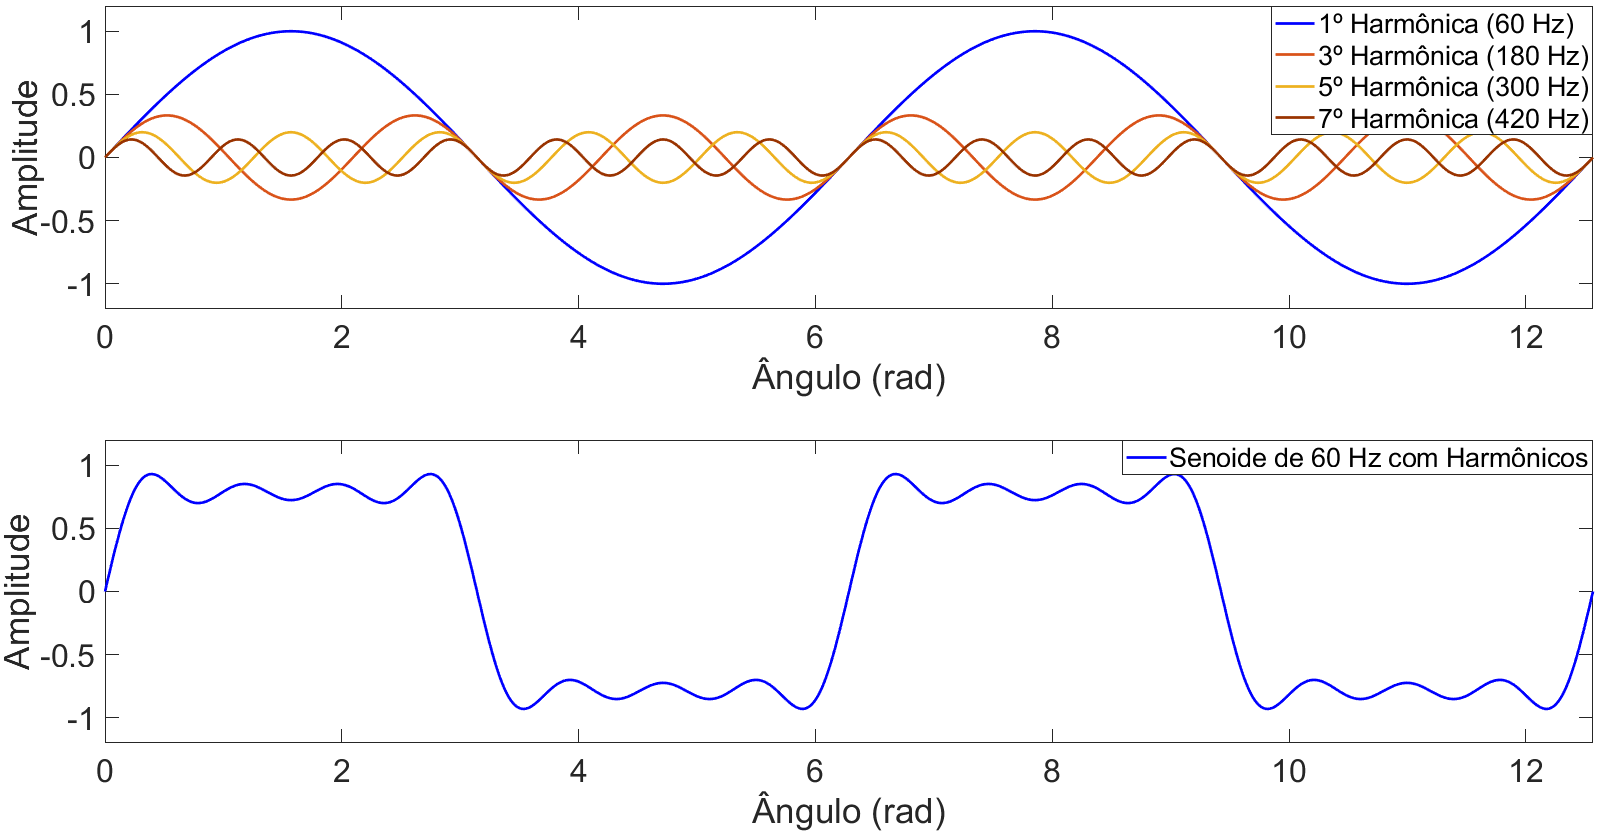
\includegraphics[scale=0.3]{img/harmonicos1.png}
\caption{\textbf{Efeito harmônico em uma senoide de 60 Hz.}}
\textbf{Fonte: Daniel Scopel (2019).}
\label{fig:Harmonicos}
\end{figure}


Também podemos utilizar o ``subfigure'' que é bem útil, veja:
\begin{figure}[H]
\centering
\subfigure[ref1][Legenda da primeira figura]{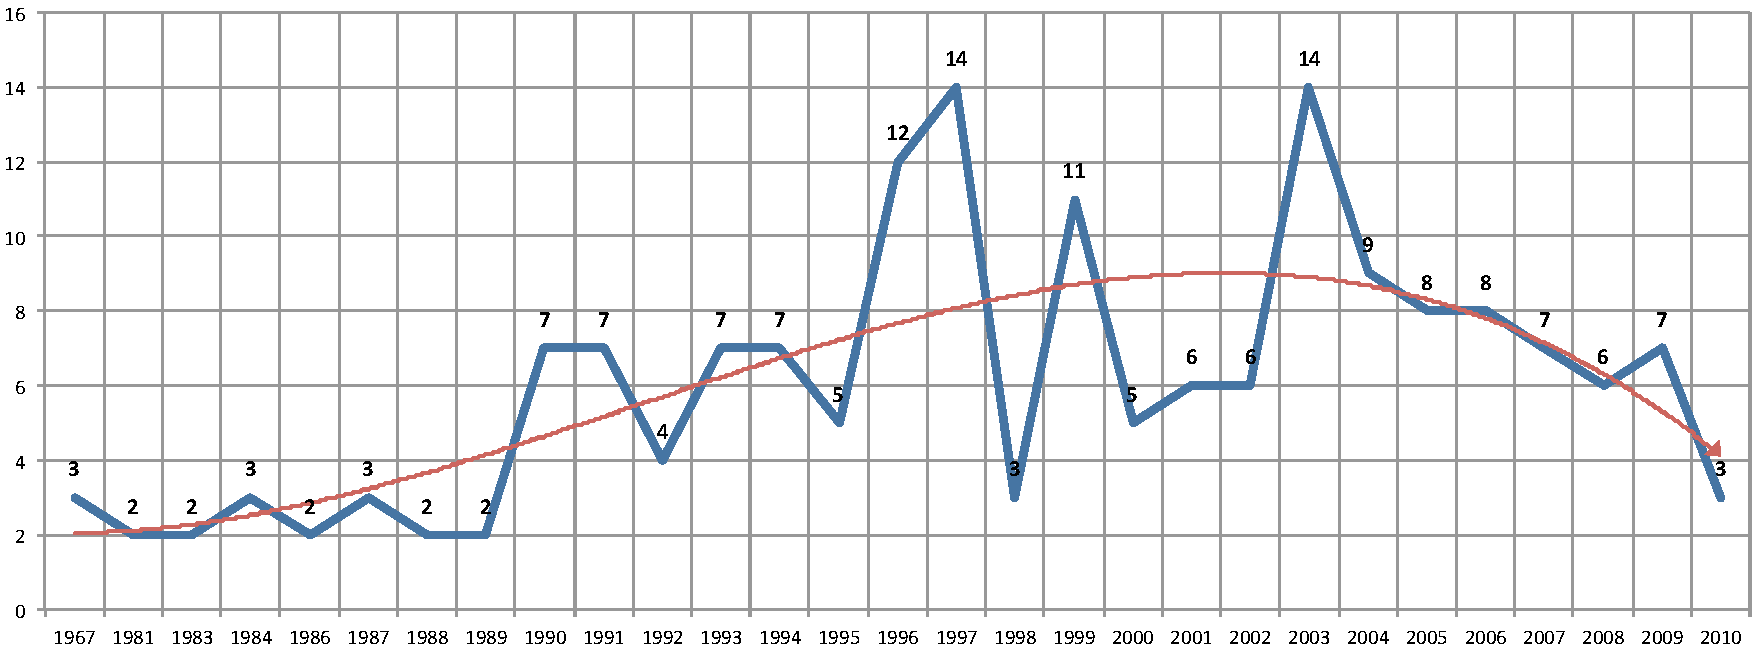
\includegraphics[width=7.52cm,height=5cm]{img/abntex2-modelo-img-grafico.pdf}}
\qquad
\subfigure[ref2][Legenda da segunda figura]{
\includegraphics[width=7.52cm,height=5cm]{img/abntex2-modelo-img-marca.pdf}}
\caption{\textbf{Legenda que engloba as duas figuras.}}
\textbf{Fonte: Daniel Scopel (2019).}
\label{fig:ondas3}
\end{figure}


\chapter{Terceiro Capítulo}
\label{chap:um_nome}

\chapter{Quarto Capítulo}
\label{chap:outro_nome}

\chapter{Conclusão}
\label{chap:conclusao}

Lembre-se que conclusão não é resumo.

\section{Trabalhos futuros}





% ----------------------------------------------------------
% ELEMENTOS PÓS-TEXTUAIS
% ----------------------------------------------------------
\postextual
% ----------------------------------------------------------

% ----------------------------------------------------------
% Referências bibliográficas
% ----------------------------------------------------------

\bibliography{Referencias}


\label{page:end}


\end{document}

